\documentclass[10pt]{article}
\usepackage[margin=0.7in,top=0.55in,bottom=0.55in]{geometry}
\usepackage{graphicx}
\usepackage{xcolor}
\usepackage{booktabs}
\usepackage{enumitem}
\usepackage{titlesec}
\usepackage[hidelinks]{hyperref}
\usepackage{array}
\usepackage{parskip}

\definecolor{accent}{HTML}{2A78D6}
\definecolor{warncol}{HTML}{EB6834}
\definecolor{inksoft}{HTML}{52514E}
\definecolor{muted}{HTML}{898781}
\definecolor{rule}{HTML}{E1E0D9}

\titleformat{\section}{\large\bfseries}{}{0pt}{}
\titlespacing*{\section}{0pt}{8pt}{3pt}
\titleformat{\subsection}{\normalsize\bfseries\color{inksoft}}{}{0pt}{}
\titlespacing*{\subsection}{0pt}{6pt}{2pt}

\setlength{\parindent}{0pt}
\setlength{\parskip}{3pt}
\pagestyle{empty}

\begin{document}

{\LARGE \bfseries AR1 Simulation Comparison --- Reference Panel at n=2000, m=4000}

\vspace{2pt}
{\color{inksoft} {\small\ttfamily n=2000, m=4000, AR1 $\rho$=0.3, $\sigma_s$=0.3, 100 reps per F$_{ST}$}}

\vspace{3pt}
\noindent\rule{\linewidth}{0.4pt}

\section*{Scope of this report}
\begin{itemize}[leftmargin=14pt, itemsep=1.5pt, topsep=1pt]
  \item Companion to the main report, scaling the \textbf{reference-panel scenarios} (originally Sections 2--3, at n=500/m=1000) up to \textbf{n=2000, m=4000} --- 4$\times$ the sample size and 4$\times$ the number of SNPs.
  \item Only the \textbf{bias-corrected} reference-panel configuration is run here (R's reference LD score matched to Python's correction, as in the original report's Figures 5--6) --- the cleanest R-vs-Python comparison. The uncorrected variant was not scaled up.
  \item Each panel compares R's two reference-panel estimators (\texttt{res\_reg\_free\_ref}, \texttt{res\_reg\_fixed\_ref}) against three Python LDSC variants: \texttt{h2\_ldsc\_nw} (free intercept, unweighted), \texttt{h2\_ldsc\_fixed\_nw} (fixed intercept, unweighted), and \texttt{h2\_ldsc\_free} --- i.e.\ \texttt{h2\_ldsc\_reg}, the standard LDSC \emph{weighted} free-intercept regression.
  \item \textbf{Implementation note:} R's reference-panel generator was rewritten to build each AR(1) column recursively ($X_{\cdot,1}\sim N(0,1)$, $X_{\cdot,j}=\rho X_{\cdot,j-1}+N(0,1-\rho^2)$) instead of via an $m\times m$ eigen-decomposition and dense matrix square root. Both constructions give the identical stationary AR(1)($\rho$) covariance ($\mathrm{Var}=1$, $\mathrm{Corr}(i,j)=\rho^{|i-j|}$); the recursive form is $O(nm)$ instead of $O(nm^2+m^3)$, which at $m=4000$ is the difference between an estimated 5+ hours and about 15 minutes per scenario with R's reference BLAS. The per-replicate in-sample LD score (unused by this comparison) was also dropped from the reference-panel scripts to avoid its $O(nm^2)$ \texttt{crossprod(X)} cost on every one of the 1100 replicates.
\end{itemize}

\section*{Reference-panel comparison at n=2000, m=4000 (bias-corrected)}

\begin{minipage}[t]{0.49\linewidth}
  \centering
  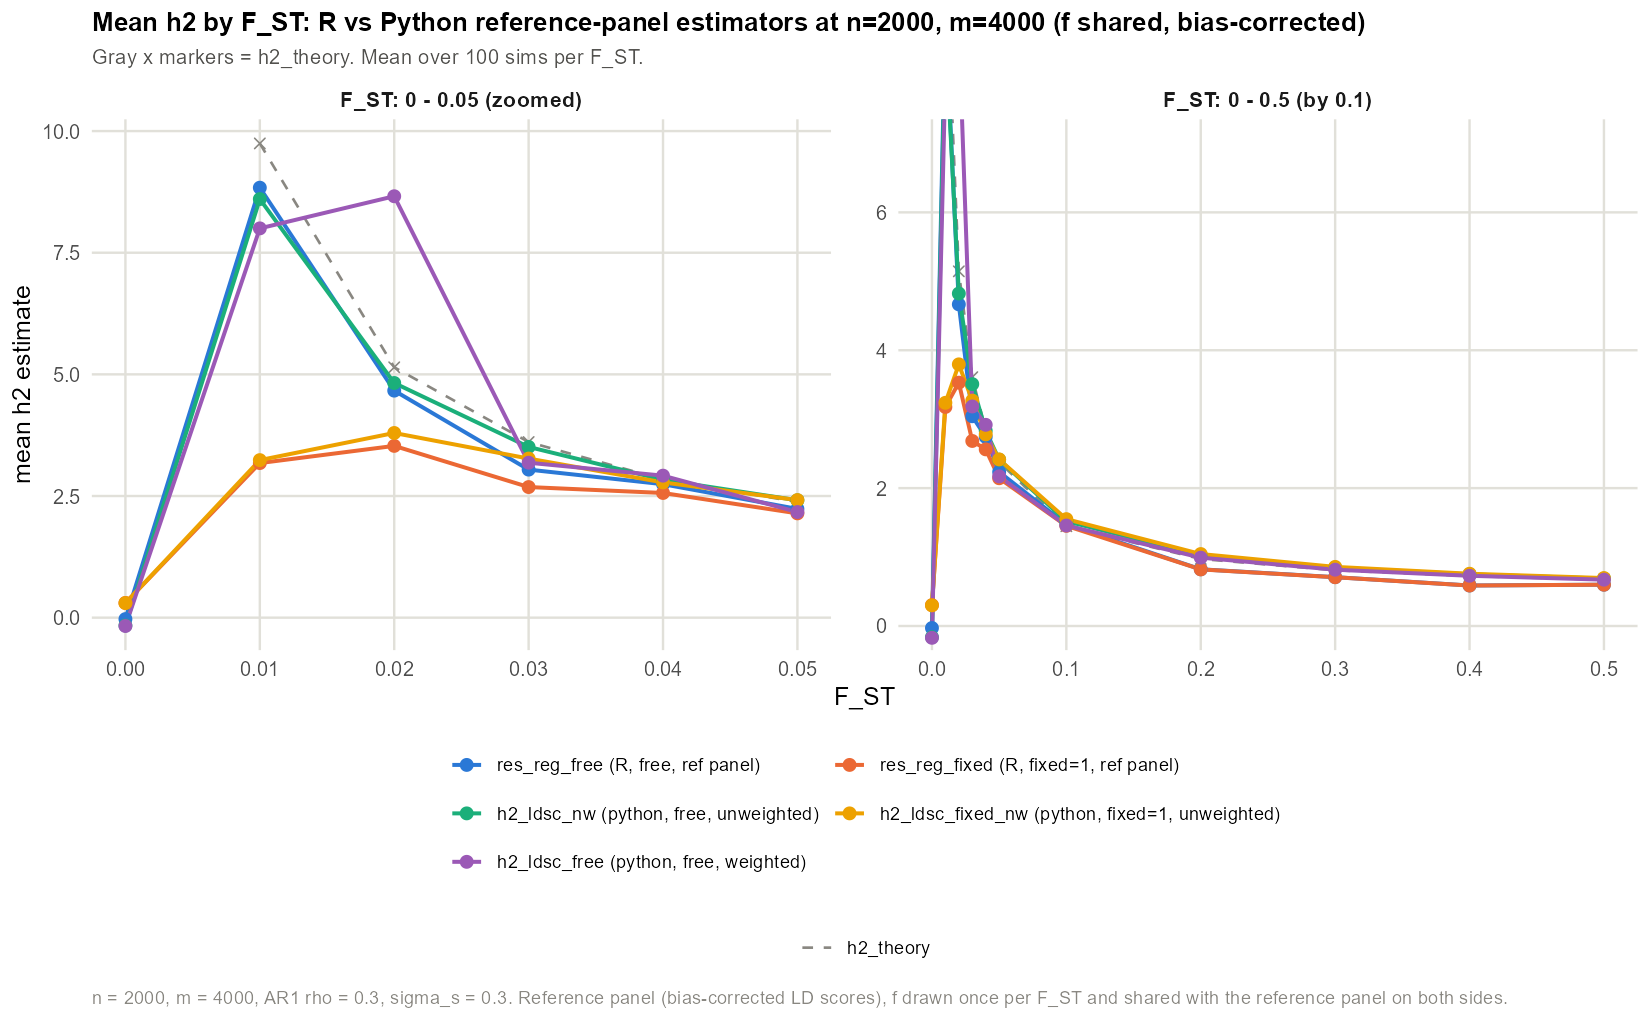
\includegraphics[width=\linewidth]{../figures/h2_by_fst_refpanel_fixedf_n2000.png}\\[2pt]
  {\footnotesize\color{inksoft}\textbf{Figure 1.} $f$ shared between the reference panel and all 100 main replicates.}
\end{minipage}
\hfill
\begin{minipage}[t]{0.49\linewidth}
  \centering
  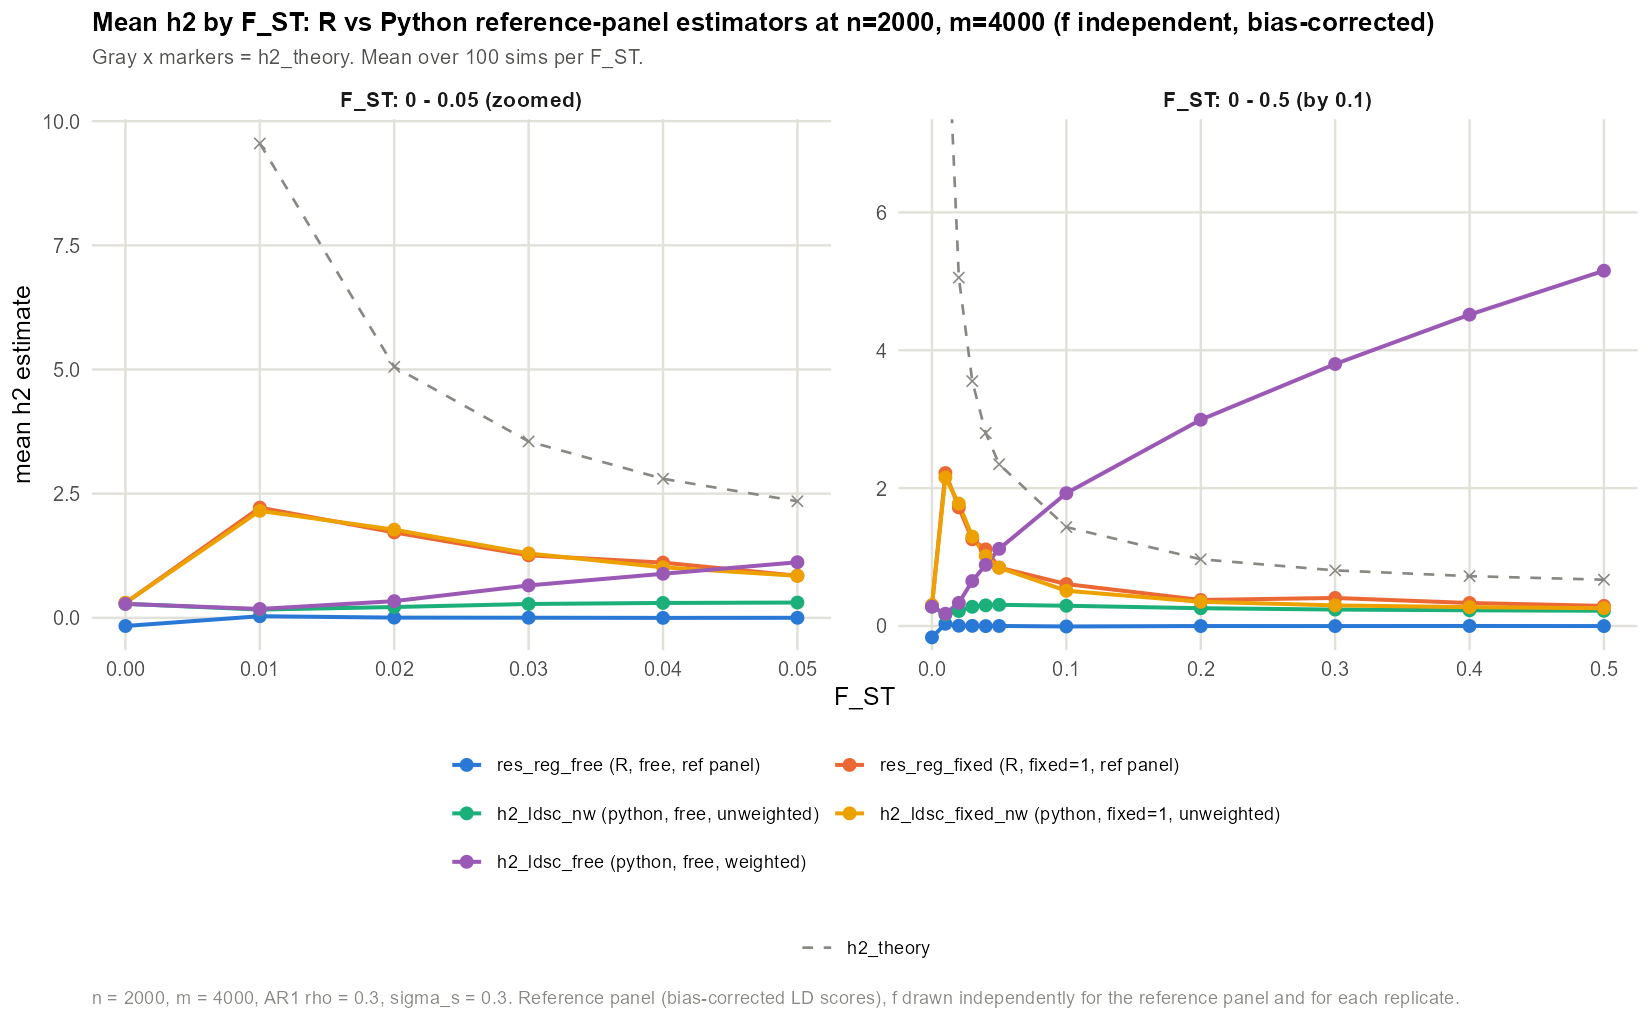
\includegraphics[width=\linewidth]{../figures/h2_by_fst_refpanel_indepf_n2000.png}\\[2pt]
  {\footnotesize\color{inksoft}\textbf{Figure 2.} $f$ drawn independently for the reference panel vs.\ each replicate.}
\end{minipage}

\vspace{4pt}
{\footnotesize\color{muted} See \texttt{report/report.tex} for the full n=500/m=1000 comparison (in-sample LD scores, the uncorrected reference-panel variant, and the diagnosis of what drove each gap) and \texttt{report/report\_ldsc\_free.tex} for the free-intercept-only n=500/m=1000 companion.}

\end{document}
